En este capítulo se introducen los actividades que permiten, a una persona interesada en extraer modelos de rendimiento a partir de una función Lambda, proceder de manera semejante a la expuesta en la Sección \ref{sec:experimento-1}. En general, se identificaron cinco apartados como los más representativos en la ejecución de este proceso, los cuales son:
\begin{enumerate}
    \item Selección del caso de uso.
    \item Instrumentalización con Kieker.
    \item Extracción del modelo con PMX.
    \item Importar archivos producidos por PMX a \emph{Palladio Workbench}.
    \item Refinamientos sobre el modelo.
\end{enumerate}

\section{Selección del caso de uso}

\begin{singlespace}
\begin{algorithm}[H]
\SetAlgoLined
%\KwResult{Write here the result }
% initialization\;
\tcc{Usuarios expertos podrían saltarse el proceso de instrumentalización y extracción}
\eIf{se cuenta con un modelo \texttt{PCM} existente}{
    utilizar este modelo para simulaciones y pruebas\;
}{
 \eIf{lenguaje en que está escrita la función es \texttt{Java}}{
    se puede utilizar la biblioteca(SDK) de \texttt{Kieker}\;
 }{
    implementar integración con \texttt{Kieker} explícitamente\;
 }
 \eIf{plataforma FaaS es \texttt{AWS Lambda}}{
     la integración con \texttt{Kieker} se da por medio de \texttt{JMS}\;
     se pueden utilizar las herramientas de monitoreo de \texttt{AWS}\;
 }{
    \tcc{La integración con Kieker podría ser similar a la propuesta o podría requerir trabajo adicional}
    implementar integración con \texttt{Kieker} explícitamente\;
    hacer uso de herramientas de medición alternas\; 
 }
}

\caption{Selección de caso de uso de función en la nube.}
\end{algorithm}
\end{singlespace}

Hoy en día se cuenta con una amplia variedad de opciones tanto en plataformas \emph{FaaS} como en lenguajes de programación que pueden ser utilizados para el desarrollo de funciones Lambda. En la Sección \ref{sec:proveedores-faas} se dan a conocer varias de estas opciones.

La selección del lenguaje de programación se hace especialmente importante si es que se desea seguir el enfoque de extracción y obtención de modelos de rendimiento expuesto en este trabajo. Al momento de escribir este documento, Java es el único lenguaje soportado por Kieker, la herramienta que gestiona la bitácora con los eventos producidos por la función Lambda.

Esto lo que quiere decir es que actualmente Kieker cuenta con bibliotecas escritas en Java que pueden ser fácilmente incluidas en el proyecto que se está desarrollando y de esta forma lograr una integración con algún servicio de bitácoras de eventos de Kieker. Si bien se puede lograr la integración entre Kieker y otro lenguaje de programación aparte de Java, esta integración deberá ser proporcionada por el implementador de forma explícita. 

La plataforma utilizada para la prueba e instalación de la función Lambda fue AWS Lambda. Como se describió en el Capítulo \ref{cap:manejador-imagenes} y en la Sección \ref{sec:experimento-1}, se hizo uso de herramientas de gestión de bitácoras (CloudWatch) y de monitoreo (AWS X-Ray) para obtener mediciones alternativas de la función, que fueron de gran ayuda a la hora de refinar el modelo de rendimiento. Si se desea implementar un caso de uso similar a \emph{Image Handler} en algún otro proveedor de servicios \emph{FaaS} (Sección \ref{sec:proveedores-faas}), se deberá  tomar en consideración las herramientas y particularidades de dicha plataforma para la obtención de mediciones de rendimiento.

El enfoque de trabajo expuesto en este documento sigue una serie de actividades que se consideran útiles para la extracción y obtención de modelos de rendimiento de una función Lambda. Estas actividades fueron adoptadas luego de estudiar la literatura pertinente y, debido a que en el presente estudio se está haciendo una exploración inicial del método de trabajo, se decidió realizar actividades de acuerdo con el orden reportado.

Implementadores con mayor experiencia en el modelado y la simulación basados en componentes podrían prescindir o modificar partes de las actividades indicadas con el fin de obtener resultados más directos de los aquí expuestos. En particular se podría:
\begin{itemize}
    \item Proporcionar un modelo en PCM \emph{a priori} de una función Lambda y de esta forma saltarse el proceso de instrumentalización y extracción.
    \item Utilizar herramientas de medición alternas para la refinamiento del modelo.
\end{itemize}

\section{Instrumentalización con Kieker}

\begin{singlespace}
\begin{algorithm}[H]
\SetAlgoLined
%\KwResult{Write here the result }
% initialization\;
\tcc{Se supone que la función Lambda está escrita en Java y será instalada en el servicio AWS Lambda}
Aprovisionar una máquina virtual en el servicio \texttt{EC2}\;
Instalar, configurar y ejecutar Kieker de acuerdo con \cite{kieker-user-guide}\;
Instalar, configurar y ejecutar una cola \texttt{JMS}\;
Configurar \texttt{Kieker} para que consuma los mensajes producidos en la cola\;

Instrumentalizar la función Lambda con el \texttt{SDK} de \texttt{Kieker}\;
Generar eventos de tipo \texttt{OperationExecutionRecord}\;
Apuntar hacia la cola \texttt{JMS} del paso 4 como el destino de los eventos de rendimiento\;

\While{ingresen invocaciones de redimensionamiento}{
      (Función $\lambda$) Publica eventos de rendimiento en la cola \texttt{JMS}\;
      (\texttt{JMS}) Gestiona los mensajes entrantes\;
      (\texttt{Kieker}) Consume mensajes de la cola y los registra en una bitácora local\;
 }
 \caption{Pasos para instrumentalizar la función con Kieker.}
\end{algorithm}
\end{singlespace}

A partir de aquí se supone que la función Lambda en la que se va a trabajar está escrita en Java y será instalada en el servicio AWS Lambda. Se tiene que descargar Kieker de \url{http://kieker-monitoring.net/}, instalarlo y ejecutarlo en una computadora en donde se pueda tener acceso y control para manipular las bitácoras obtenidas. Se recomienda la lectura del manual de usuario de Kieker, disponible en \cite{kieker-user-guide}, para obtener mayores detalles referentes a su instalación y configuración.

Kieker permite varias formas de configuración y ejecución. Debido a que las funciones Lambda se ejecutan en ambientes que son inaccesibles por los implementadores, se optó por configurar Kieker para que escuche los eventos de la función por medio de una cola JMS. La cola JMS y el servicio de Kieker fueron instalados y configurados en una máquina virtual independiente.

En la Sección \ref{sec:image-handler-kieker-pmx} se introdujo la programación requerida para generar entradas en una bitácora de Kieker. Se generaron eventos de tipo \emph{OperationExecutionRecord} que son los tipos de registros más básicos que se pueden producir en Kieker y, además, se configuró la biblioteca de Kieker para que publicara los eventos de rendimiento a una cola JMS. El servicio de Kieker consume los eventos de la cola y los registra en una bitácora local.

%\begin{center}
%Función Lambda $\rightarrow$ JMS $\rightarrow$ Kieker $\rightarrow$ Bitácora
%\end{center}

Se recomienda la lectura del manual de usuario y del tutorial de Kieker disponibles en \cite{kieker-user-guide} y en \cite{kieker-icpe-tutorial-2014} respectivamente, para tener mayores detalles sobre otros tipos de eventos que pueden ser generados por la biblioteca de Kieker.

\section{Extracción del modelo con PMX}

\begin{singlespace}
\begin{algorithm}[H]
\SetAlgoLined
%\KwResult{Write here the result }
% initialization\;

Descargar e instalar \texttt{PMX}\;
\eIf{se ejecuta con \texttt{Docker}}{
    Ir al directorio \texttt{pcmserver}\;
    Iniciar el contenedor \texttt{Docker}\;
    Ir al navegador, acceder a \texttt{pmx-pcm-server}\;
    Subir una bitácora de \texttt{Kieker} y analizarla\;
}{
    \If{se ejecuta \texttt{pcmConsole.jar}}{
        Ir al directorio \texttt{pcmserver}\;
        Ejecutar \texttt{pcmConsole.jar}\;
        Revisar directorio destino con los archivos producidos\;            
    }
}
\If{\texttt{PMX} no genera archivos de \texttt{PCM}}{
    Revisar la instrumentalización de \texttt{Kieker}\;
    Revisar el manual de usuario de \texttt{Kieker}\;
}
\caption{Extracción de un modelo de rendimiento con PMX.}
\end{algorithm}
\end{singlespace}


Se debe descargar PMX del sitio Web \url{https://se.informatik.uni-wuerzburg.de/software-engineering-group/tools/pmx/}. Una vez obtenida la distribución de PMX, hay que asegurarse de usar la versión de PMX que extrae modelos de rendimiento en PCM, \texttt{pcm-pmx}, esto debido a que PMX puede generar modelos de rendimiento en PCM y DML (Sección \ref{sec:dml}) y ambas versiones vienen incluidos en el archivo que se descarga.

Una vez que se cuenta con la versión \texttt{pcm-pmx}, existen dos opciones para extraer un modelo de rendimiento PCM a partir de una bitácora en Kieker:
\begin{enumerate}
    \item Ejecutar \texttt{pcm-pmx-server}, la aplicación Web que proporciona el servicio de extracción a partir de una bitácora de Kieker, como un contenedor Docker.
    \item Ejecutar \texttt{pcmConsole.jar}, la aplicación Java que lleva a cabo el trabajo de extracción del modelo PCM a partir de una bitácora en Kieker.
\end{enumerate}

Con ambas herramientas se puede extraer un modelo PCM a partir de una bitácora de Kieker. Con \texttt{pcm-pmx-server} se puede acceder a una página Web, la cual provee un formulario para subir una bitácora, analizarla y luego obtener un archivo \texttt{.zip} con los resultados de la extracción. Si se utiliza \texttt{pcmConsole.jar} es un método más directo. Se invoca al programa con los siguientes parámetros:
\begin{itemize}
    \item La ruta en donde se encuentra la bitácora de Kieker.
    \item La ruta en donde se desea almacenar los archivos resultantes de la extracción del modelo.
\end{itemize}
Ambas herramientas no son excluyentes entre sí.  \texttt{pcm-pmx-server} usa \texttt{pcmConsole.jar} para el ejecutar el proceso de extracción.

\subsection{\texttt{pcm-pmx-server} con Docker} 
Al momento de escribir este documento \texttt{pcm-pmx-server} se encuentra bajo la siguiente ruta (suponemos ``\texttt{pmx}'' como el directorio padre, el directorio principal de la distribución descargada de \texttt{pmx}):
\begin{verbatim}
pmx/pmx-pcm/tools.descartes.pmx.pcm.docker/pcmserver
\end{verbatim}
Una vez dentro del directorio \texttt{pcmserver}, ejecutar los siguientes comandos para iniciar el contenedor Docker:

\begin{verbatim}
> docker build -t descartesresearch/pmx-pcm-server .
> docker run -d -p 8080:8080 descartesresearch/pmx-pcm-server
# para detener el contendor
> docker stop {id-de-contenedor}
\end{verbatim}

\begin{figure}[h]
  \centering
  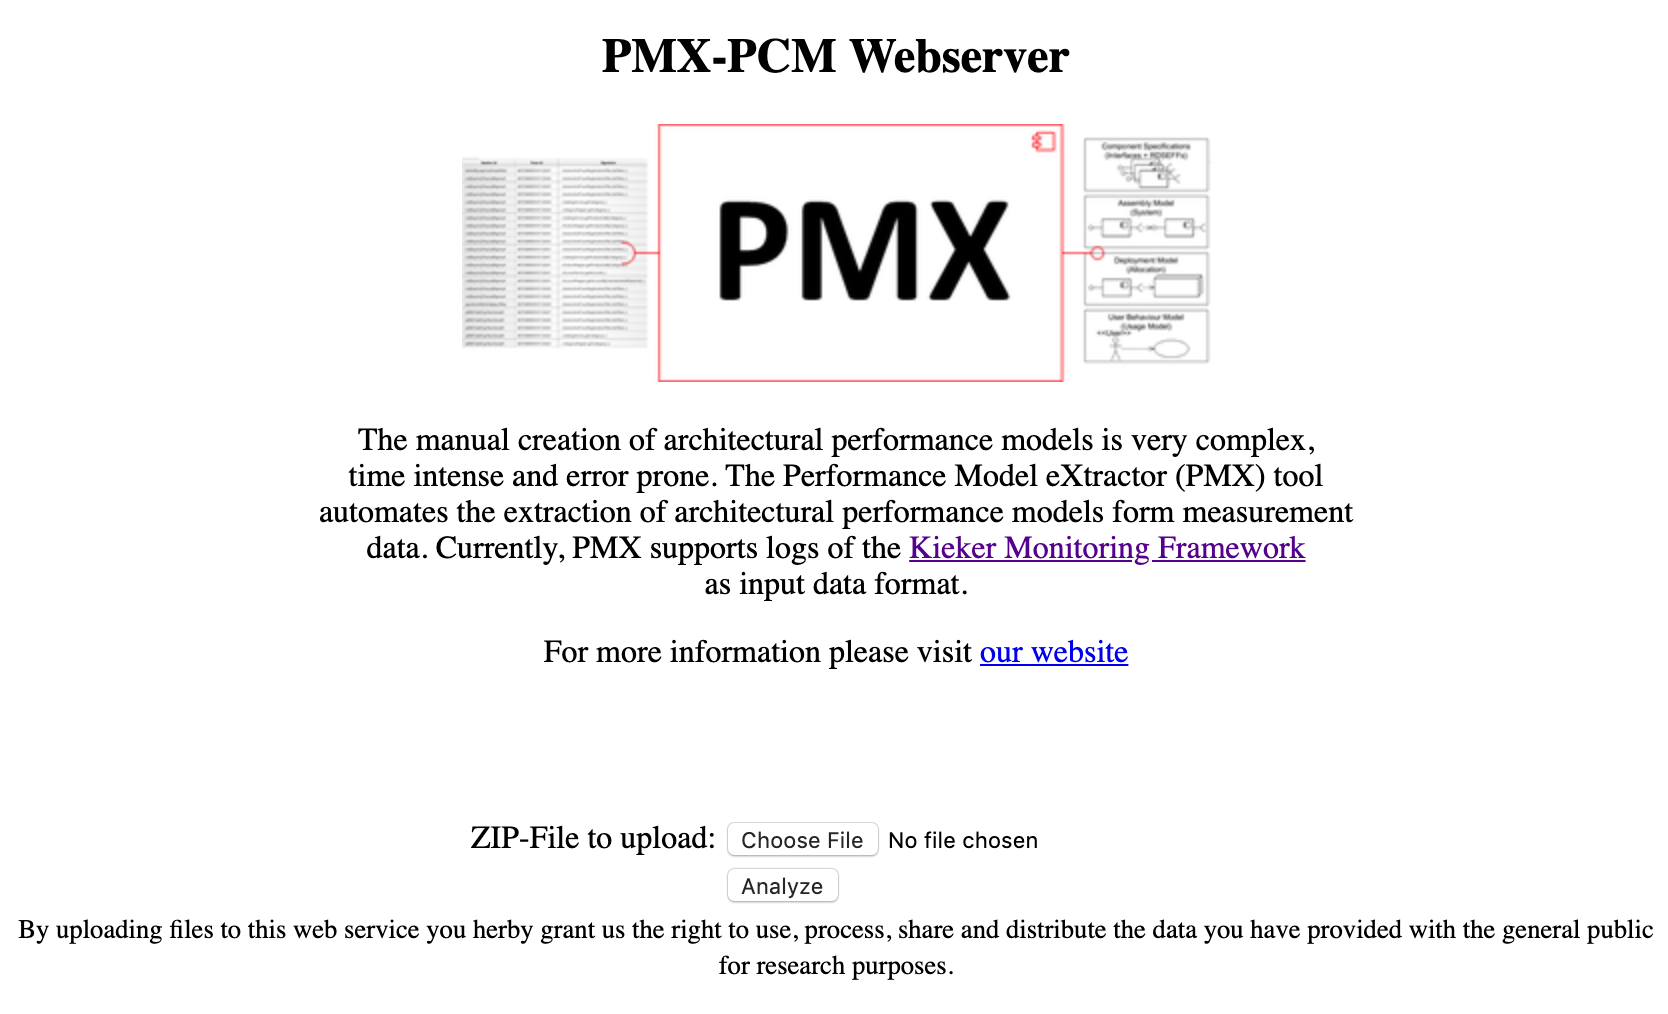
\includegraphics[width=15cm]{pcmserver}
  \caption{PMX-PCM Server. Tomado del Sitio Web de PMX.}
  \label{fig:pcmserver}
\end{figure}

La figura \ref{fig:pcmserver} muestra el formulario proporcionado por el PCX-PCM WebServer para extraer un modelo PCM a partir de una bitácora en Kieker.

\subsection{Extracción con \texttt{pcmConsole.jar}} Al momento de escribir este documento \texttt{pcmConsole.jar} se encuentra bajo la siguiente ruta (suponemos ``\texttt{pmx}'' como el directorio padre, el directorio principal de la distribución descargada de \texttt{pmx}):
\begin{verbatim}
pmx/pmx-pcm/tools.descartes.pmx.pcm.docker/pcmserver/pcmConsole.jar
\end{verbatim}
Una vez dentro del directorio \texttt{pcmserver}, se puede ejecutar el siguiente comando:

\begin{verbatim}
java -jar pcmConsole.jar -i <ruta-directorio-de-bitacora> \
    -o <ruta-directorio-destino>
\end{verbatim}

\subsubsection{Consideraciones}
Si PMX no entrega ningún resultado como parte del proceso de extracción, esto quiere decir que la bitácora proporcionada no tiene un formato apropiado para PMX. Si esto pasa, vale la pena revisar los puntos en donde se introdujo la instrumentación de Kieker. Se debe revisar si los eventos contienen toda la información necesaria de acuerdo con el manual de usuario. 

\subsection{Importar archivos producidos por \texttt{PMX} a \emph{Palladio Workbench}}
\begin{singlespace}
\begin{algorithm}[H]
\SetAlgoLined
%\KwResult{Write here the result }
% initialization\;
\tcc{Se supone que se ha logrado obtener un modelo PCM por medio de PMX}
Crear nuevo proyecto en \emph{Palladio Workbench}\;
Importar archivos generados por \texttt{PMX}\;
\eIf{archivos son compatibles con Palladio Workbench}{
    Iniciar con la ejecución de simulaciones\;
}{
    Evaluar incompatibilidades y corregir\;
}
\caption{Importación de archivos de PMX an \emph{Palladio Workbench}.}
\end{algorithm}
\end{singlespace}

Si el proceso anterior se realizó con éxito, PMX  generará 5 archivos en formato XML que representan cada uno de los modelos con los que se puede trabajar en Palladio: modelo de componentes, asignación de recursos, ambiente, sistema y uso. También se generan archivos \texttt{*.csv} con estimaciones del uso de los componentes. El uso de las estimaciones contenidas en estos archivos es opcional, puesto que en la Sección \ref{sec:experimento-1} explicamos una alternativa que nos brindó mayor precisión.

En \emph{Palladio Workbench} hay que crear un nuevo proyecto y ponerle un nombre.
\begin{verbatim}
File > New > Project > Other > New Palladio Project
\end{verbatim}
Luego de esto hay que importar cada uno de los archivos XML producidos por PMX al proyecto recién creado.
\begin{verbatim}
Seleccionar el proyecto > 
File > Import > File System > Seleccionar el directorio con los archivos
\end{verbatim}
Con los archivos cargados en el proyecto, se puede entonces iniciar la ejecución de simulaciones.
\begin{verbatim}
Seleccionar el proyecto > Click derecho > Run As > Run Configurations
\end{verbatim}
Luego se muestra la pantalla en donde se crean y administran configuraciones de ejecución. En este estudio se utilizó el motor de simulación \texttt{SimuBench} pero se proveen otros motores de simulación. Se puede utilizar los valores por defecto en un inicio y, por último, ejecutar las simulaciones.


\subsubsection{Consideraciones}
\begin{enumerate}
    \item Los espacios de nombres, \emph{namespaces}, de los archivos XML producidos por PMX pueden llegar a ser diferentes a los de la versión de \emph{Palladio Workbench} que se esté utilizando. Dependiendo del modelo PCM con el que se esté trabajando esto podría llegar a ser un problema. 
    \item Algunos tipos de datos producidos en los archivos XML de PMX pueden llegar a ser diferentes a los de la versión de \emph{Palladio Workbench}.
\end{enumerate}

Un ajuste que ayudó a resolver estos problemas de compatibilidad, fue generar un nuevo proyecto en \emph{Palladio Workbench} y utilizar, por ejemplo, en el modelo de repositorio, componentes similares a los producidos por PMX. Luego ver el código XML del modelo de repositorio y comparar las definiciones de este archivo con el de PMX.
 
\subsection{Refinamientos sobre el modelo}
\begin{singlespace}
\begin{algorithm}[H]
\SetAlgoLined
%\KwResult{Write here the result }
% initialization\;
\tcc{Se supone que se cuenta con modelo PCM válido}
Ejecutar simulaciones con \emph{SimuBench}\;
\Repeat{los resultados sean satisfactorios}{
    Modificar submodelos\;
    Obtener estimaciones de herramientas alternas a \texttt{PMX}\;
    Evaluar resultados\;
}
\caption{Ejecución de simulaciones y refinamiento del modelo.}
\end{algorithm}
\end{singlespace}

Una vez que se cuenta con el modelo PCM, se puede iniciar la ejecución de simulaciones. Conforme se van dando las ejecuciones, el motor de simulaciones de PCM (en este caso SimuBench) entrega 6 tipos de visualización de resultados para cada uno de los componentes identificados. También incluye estimaciones de la demanda del procesador y del disco duro. En este trabajo fueron de particular utilidad las visualizaciones de resultados de tipo: \texttt{XY Plot}, histograma y función de distribución acumulada.

Los resultados entregados por el motor de simulaciones vienen dados en tiempos de respuesta en segundos. Si los resultados de las simulaciones están muy alejados de los observados en invocaciones reales, se recomienda modificar el modelo en alguno de sus submodelos asociados. Una de las desventajas que se experimentó con el modelo obtenido por PMX fueron las estimaciones de las demandas de los recursos, esto se explica con mayor detalle en la Sección \ref{sec:experimento-1}. Para lidiar con esto, fue necesario hacer uso de herramientas alternas con el fin de afinar estas estimaciones, para luego repetir las simulaciones hasta que los resultados obtenidos se consideraron relevantes. En este estudio, la herramienta AWS X-Ray fue sumamente útil para llevar a cabo tal labor. 

%También se realizaron modificaciones sobre el modelo de uso para generar cargas de trabajo con comportamientos similares a los hechos en las invocaciones reales.

La Sección \ref{sec:experimento-1} brinda un mayor detalle acerca de la estrategia de afinamiento del modelo de rendimiento para el caso de \emph{Image Handler} pero, en términos generales, una vez obtenido un modelo, todo dentro de él está sujeto a modificación y evaluación. La literatura consultada hace énfasis en esto y, para el caso de \emph{Image Handler} esto no fue la excepción. Llegado a este punto, se entra en un ciclo de prueba $\rightarrow$ validación $\rightarrow$ afinamiento del modelo hasta que los resultados obtenidos por medio de las simulaciones resulten significativas para el caso de estudio en particular.

